Empezaremos mencionando y caracterizando algunas familias de grafos
para las que nuestra heurist\'ica golosa constructiva siempre encuentra
un resultado correcto, esto es, una clique de m\'axima frontera.

Teniendo en cuenta, como ya se menciono anteriormente, que la heur\'istica
empieza por uno de los nodos de mayor grado y en cada paso va 
agregando nodos que forman clique con los nodos actualmente escogidos
bajo la condici\'on de que el grado de los mismos sea mayor a dos veces
el tama\~no de la clique actual (de estos candidatos, tambi\'en elige
uno de los de mayor grado). Tenemos lo siguiente:

En todos los casos en los que hay varios candidatos para agregar a la
clique con el mismo grado (en particular el primero) la heur\'istica
puede proporcionar el resultado incorrecto, dado que el algoritmo
elige determin\'isticamente uno de los candidatos mientras que la 
entrada es aleatoria (la idea es poder resolver el problema para
cualquier grafo de entrada), veremos a continuaci\'on que excepto
en casos muy particulares, grafos isomorfos cuyas matrices de adyacencia
son distintas pueden, al ser sometidos a la heur\'istica, arrojar
resultados muy dispares (en particular, resultados correctos, versus
resultados incorrectos).

\subsubsection{Grafos completos}
	\begin{center}
		\begin{tabular}{ |c||c| }
			\hline
			Grafo de entrada & Paso 1 \\
			\hline\hline
			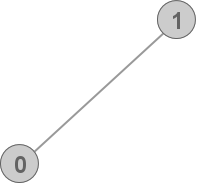
\includegraphics[scale = 0.3]{img/ej3/constructiva_golosa/K2_st0.png} &
			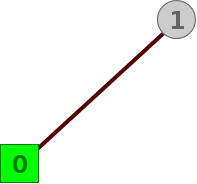
\includegraphics[scale = 0.3]{img/ej3/constructiva_golosa/K2_st1.png} \\
			\hline
			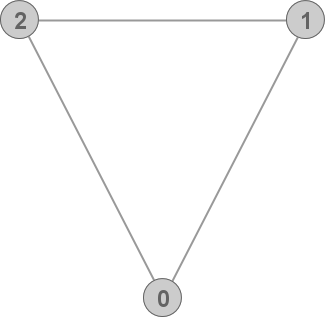
\includegraphics[scale = 0.3]{img/ej3/constructiva_golosa/K3_st0.png} &
			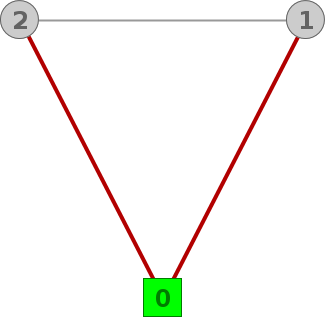
\includegraphics[scale = 0.3]{img/ej3/constructiva_golosa/K3_st1.png} \\
			\hline
		\end{tabular}
		\begin{tabular}{ |c||c||c| }
			\hline
			Grafo de entrada & Paso 1 & Paso 2 \\
			\hline\hline
			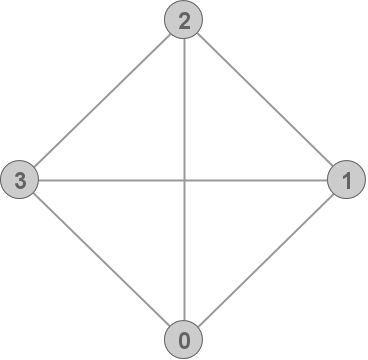
\includegraphics[scale = 0.3]{img/ej3/constructiva_golosa/K4_st0.png} &
			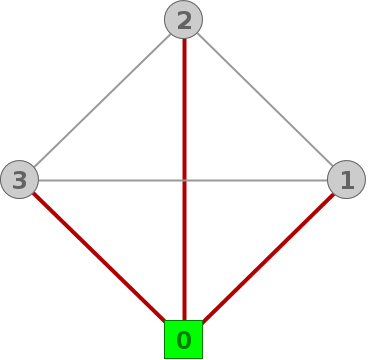
\includegraphics[scale = 0.3]{img/ej3/constructiva_golosa/K4_st1.png} &
			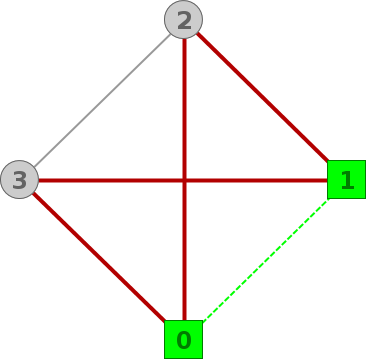
\includegraphics[scale = 0.3]{img/ej3/constructiva_golosa/K4_st2.png} \\
			\hline
			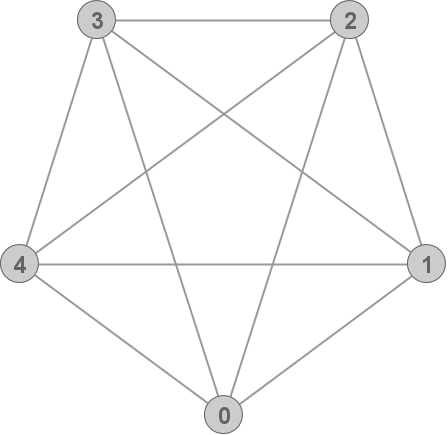
\includegraphics[scale = 0.3]{img/ej3/constructiva_golosa/K5_st0.png} &
			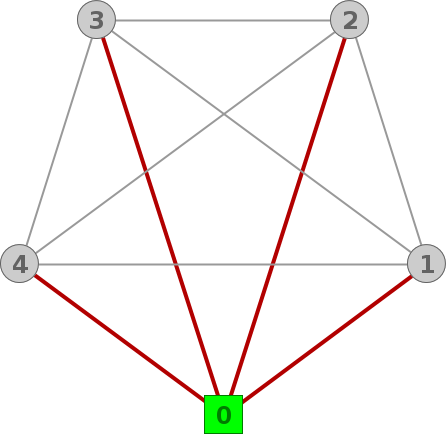
\includegraphics[scale = 0.3]{img/ej3/constructiva_golosa/K5_st1.png} &
			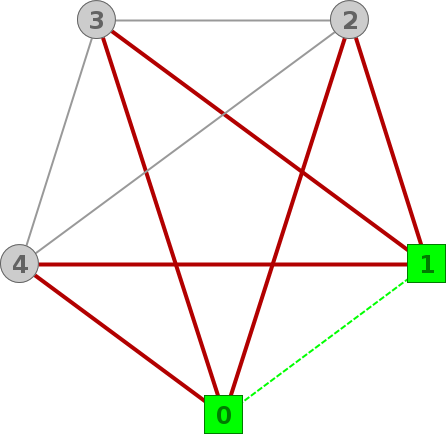
\includegraphics[scale = 0.3]{img/ej3/constructiva_golosa/K5_st2.png} \\
			\hline
		  \end{tabular}
		  \begin{tabular}{ |c||c||c||c| }
			\hline
			Grafo de entrada & Paso 1 & Paso 2 & Paso 3 \\
			\hline\hline
			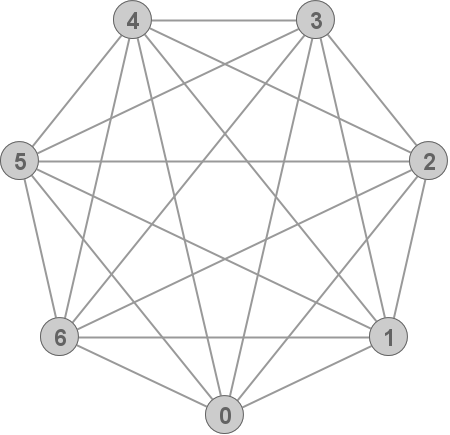
\includegraphics[scale = 0.25]{img/ej3/constructiva_golosa/K7_st0.png} &
			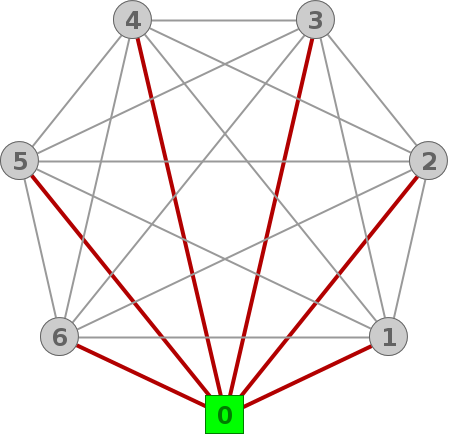
\includegraphics[scale = 0.25]{img/ej3/constructiva_golosa/K7_st1.png} &
			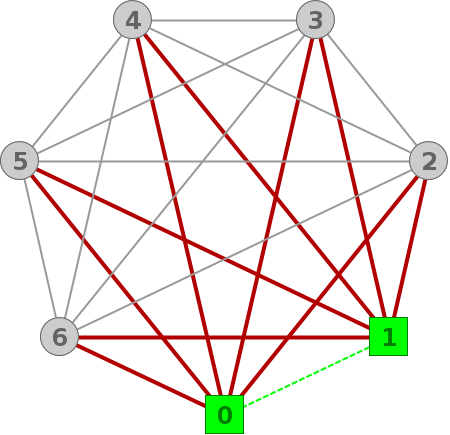
\includegraphics[scale = 0.25]{img/ej3/constructiva_golosa/K7_st2.png} &
			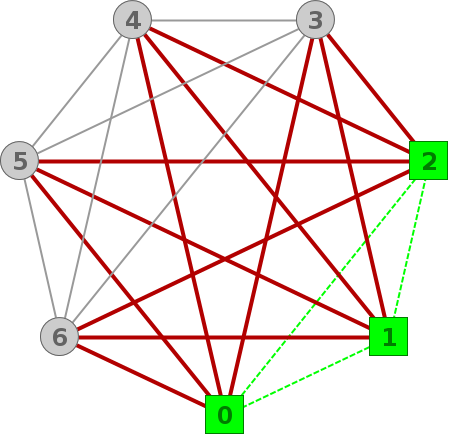
\includegraphics[scale = 0.25]{img/ej3/constructiva_golosa/K7_st3.png} \\
			\hline
		\end{tabular}
	\end{center}

	En estos grafos como ya se mencion\'o anteriormente, el algoritmo
	escoge nodos y va haciendo crecer una clique hasta llegar a una 
	clique de tama\~no $n/2$, notes\'e que todos los nodos en los 
	grafos de esta familia tienen grado $d(i) = n - 1$, por lo
	tanto la selecci\'on en cada paso del siguiente nodo de la
	clique es dependiente de la implementaci\'on

	Tambi\'en anal\'iticamente puede verse que las CMF para esta 
	familia de grafos son tanto las $K_{\left \lfloor{n/2}\right \rfloor}$ 
	como las $K_{\left \lceil{n/2}\right \rceil}$. Habiendo establecido como
	cota superior al tama\~no de la CMF el valor $n/2$, la posibilidad de que
	los $K_{\left \lceil{n/2}\right \rceil}$ tambi\'en cumplan parece una 
	anomal\'ia a priori. Veremos que no lo es y que est\'a directamente
	relacionado con la naturaleza de la familia en estudio. 

	La frontera es la cantidad de aristas que sale de cada uno de los
	nodos de la clique hacia nodos que no est\'an en la misma. Siendo
	$n$ la cantidad de nodos del grafo y habiendo establecido que la CMF
	tiene tama~no $\left \lfloor{n/2}\right \rfloor$, 
	si la clique en estudio tiene este tama\~no, los nodos que quedan afuera
	de la clique son $\left \lceil{n/2} \right \rceil$, luego: 

	\( 
	\delta(K_{\left \lfloor{n/2}\right \rfloor}) = 
	\left \lfloor{n/2} \right \rfloor \times 
	(n - \left \lfloor{n/2} \right \rfloor ) = 
	\left \lfloor{n/2} \right \rfloor \times 
	(\left \lfloor{n/2} \right \rfloor +
	\left \lceil{n/2} \right \rceil - 
	\left \lfloor{n/2} \right \rfloor) =
	\left \lfloor{n/2} \right \rfloor \times
	\left \lceil{n/2} \right \rceil = 
	\delta(K_{\left \lceil{n/2}\right \rceil})
	\)
\begin{figure}[H]
\caption{Ejemplos grafos completos - Entrada / Salida}
\centering
%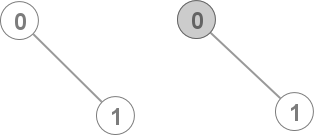
\includegraphics[scale = 0.5]{img/ej3/constructiva_golosa/k2.png}
%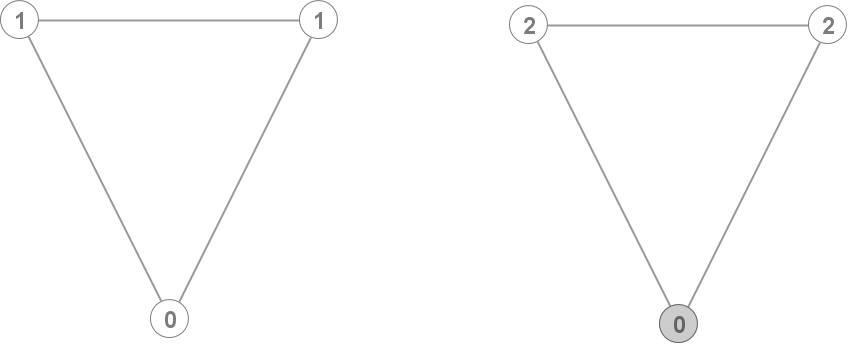
\includegraphics[scale = 0.5]{img/ej3/constructiva_golosa/k3.png}
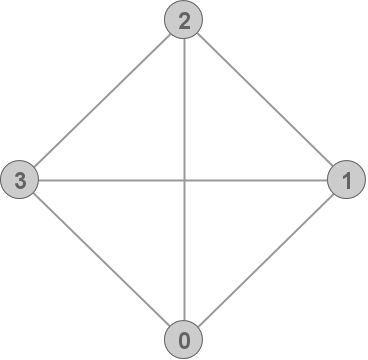
\includegraphics[scale = 0.5]{img/ej3/constructiva_golosa/K4_st0.png}
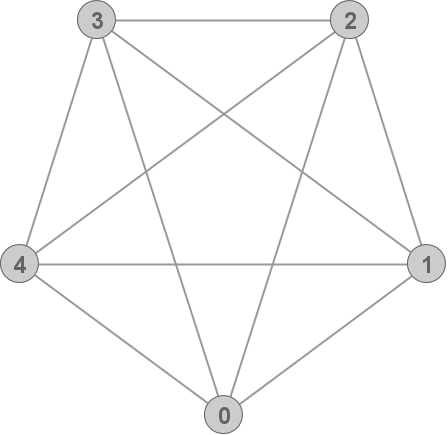
\includegraphics[scale = 0.5]{img/ej3/constructiva_golosa/K5_st0.png}
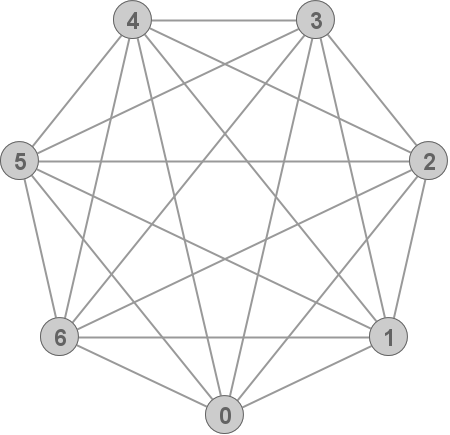
\includegraphics[scale = 0.5]{img/ej3/constructiva_golosa/K7_st0.png}
\end{figure}

\subsection{\'Arboles}
La familia de los \'arboles es una de las familias en las que la heur\'istica
se puede romper y no devolver el resultado correcto. 

Para los \'arboles es pr\'acticamente inmediato que el 
tama\~no de la clique de m\'axima frontera es a lo sumo igual a dos, dado
que por su misma definici\'on los arboles no contienen circuitos simples.

Nuevamente en este caso se toma alguno de los nodos de mayor grado 
y se intenta hacer crecer la clique con alg\'un nodo adyacente.

Como puede verse en los siguientes ejemplos en el caso de que 
implementativamente se seleccione uno de los nodos de mayor grado
adyacente a otro de los nodos de mayor grado, la heur\'istica encuentra
efectivamente una CMF, pero en el caso de que el nodo de partida sea 
uno de los de mayor grado en el grafo y dicho nodo no pertenezca a
ninguna de las CMF del grafo, la heur\'istica reportar\'a un falso 
positivo (una clique cuya frontera es maximal pero no m\'axima).

Desde un punto de vista implementativo el desempate entre nodos de 
mismo grado, depender\'a de la matriz de adyacencia (la posici\'on en
la que aparece un nodo) y dado que existe un arbol isomorfo al del 
ejemplo en el que el nodo incorrecto para empezar la clique est\'a
listado antes que el nodo correcto (el que permite generar la CMF),
el siguiente es un buen ejemplo para ilustrar la fragilidad de la
heur\'istica

\begin{figure}[H]
\caption{Ejemplos \'Arboles}
\centering
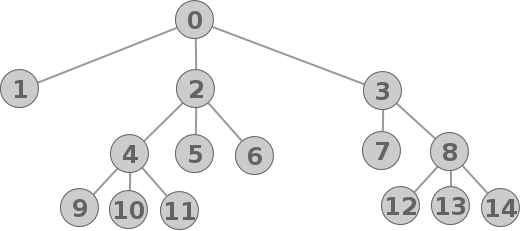
\includegraphics[scale = 0.5]{img/ej3/constructiva_golosa/tree_st0.png}
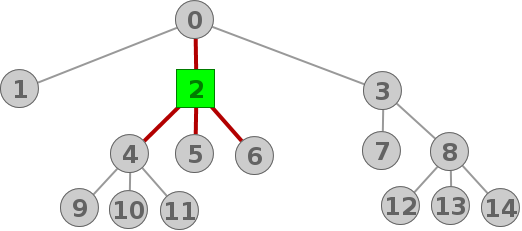
\includegraphics[scale = 0.5]{img/ej3/constructiva_golosa/tree_st01.png}
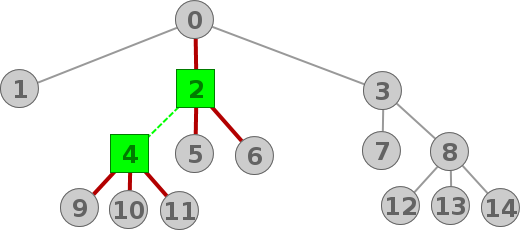
\includegraphics[scale = 0.5]{img/ej3/constructiva_golosa/tree_st02.png}
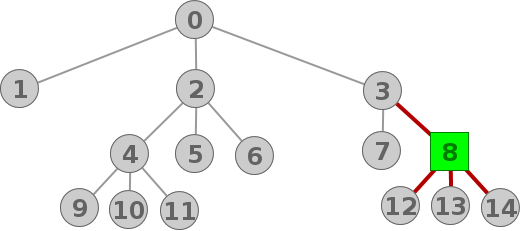
\includegraphics[scale = 0.5]{img/ej3/constructiva_golosa/tree_st11.png}
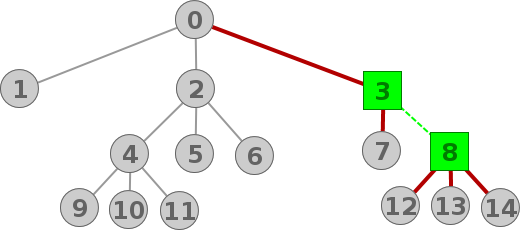
\includegraphics[scale = 0.5]{img/ej3/constructiva_golosa/tree_st12.png}
\end{figure}

	\begin{center}
		\begin{tabular}{ |c||c||c| }
			\hline
			Grafo de entrada & Paso 1 & Paso2 \\
			\hline\hline
			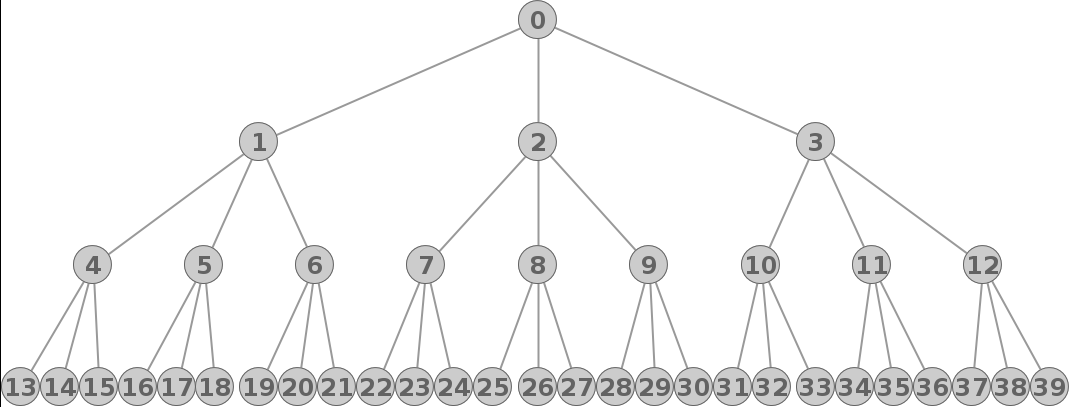
\includegraphics[scale = 0.15]{img/ej3/constructiva_golosa/ctree_st0.png} &
			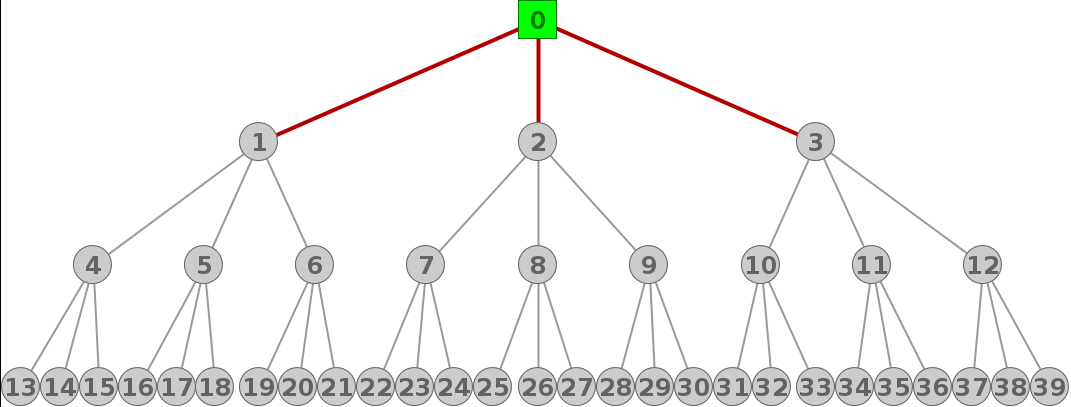
\includegraphics[scale = 0.15]{img/ej3/constructiva_golosa/ctree_st1.png} &
			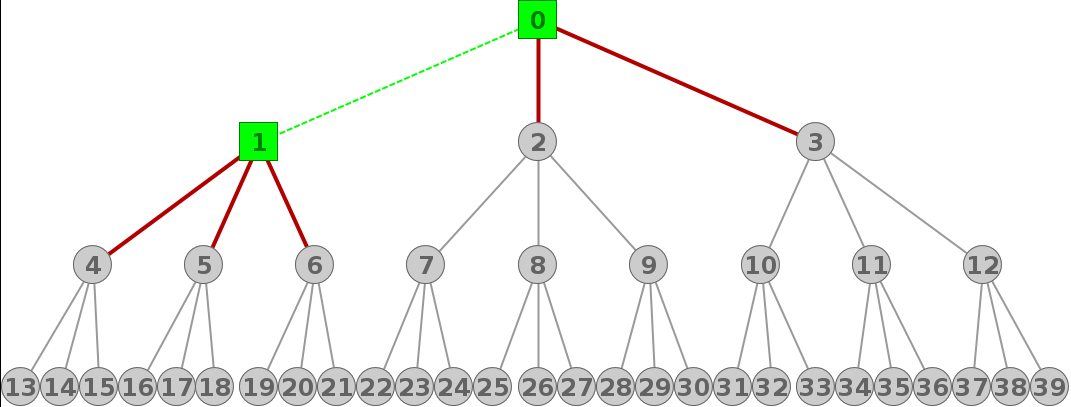
\includegraphics[scale = 0.15]{img/ej3/constructiva_golosa/ctree_st2.png} \\
			\hline
			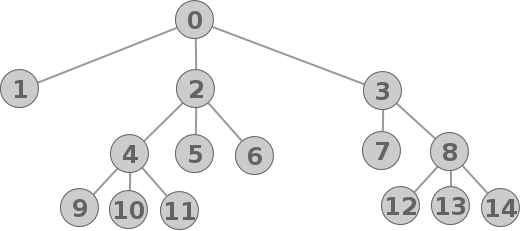
\includegraphics[scale = 0.3]{img/ej3/constructiva_golosa/tree_st0.png} &
			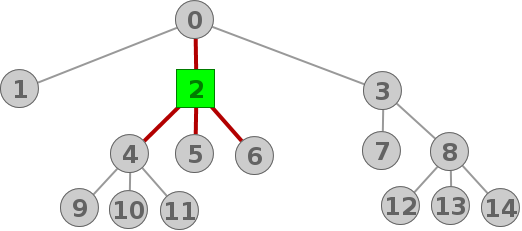
\includegraphics[scale = 0.3]{img/ej3/constructiva_golosa/tree_st01.png} &
			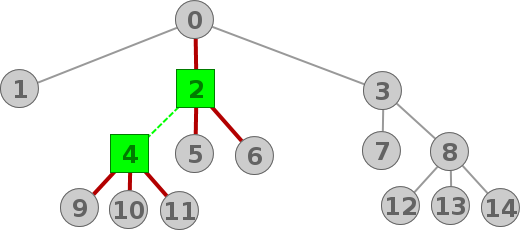
\includegraphics[scale = 0.3]{img/ej3/constructiva_golosa/tree_st02.png} \\
			\hline
			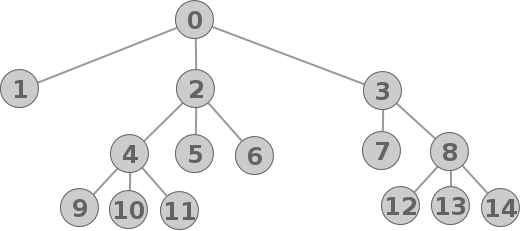
\includegraphics[scale = 0.3]{img/ej3/constructiva_golosa/tree_st0.png} &
			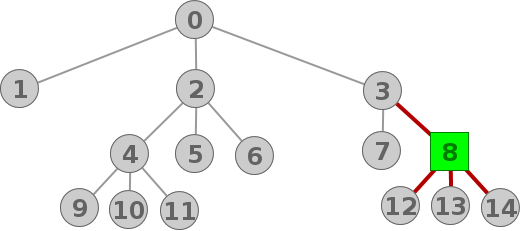
\includegraphics[scale = 0.3]{img/ej3/constructiva_golosa/tree_st11.png} &
			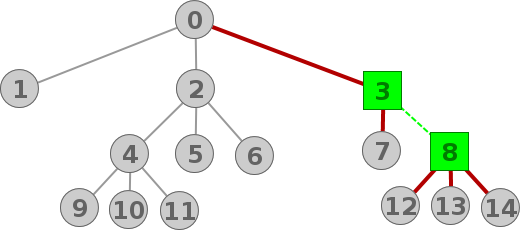
\includegraphics[scale = 0.3]{img/ej3/constructiva_golosa/tree_st12.png} \\
			\hline
		\end{tabular}
	\end{center}
			
\subsection{Grafos bipartitos}
	\begin{center}
		\begin{tabular}{ |c||c||c| }
			\hline
			Grafo de entrada & Paso 1 & Paso2 \\
			\hline\hline
			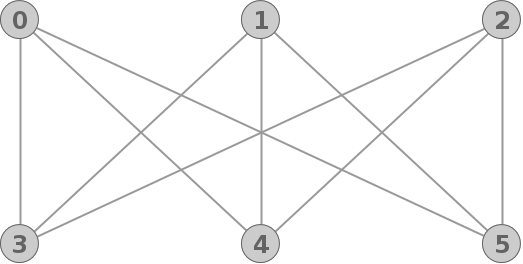
\includegraphics[scale = 0.2]{img/ej3/constructiva_golosa/k3,3_st0.png} &
			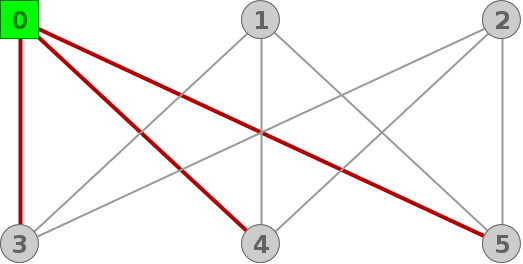
\includegraphics[scale = 0.2]{img/ej3/constructiva_golosa/k3,3_st1.png} &
			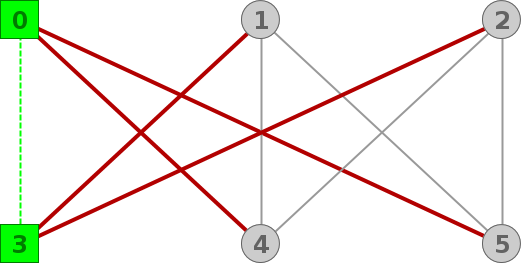
\includegraphics[scale = 0.2]{img/ej3/constructiva_golosa/k3,3_st2.png} \\
			\hline
			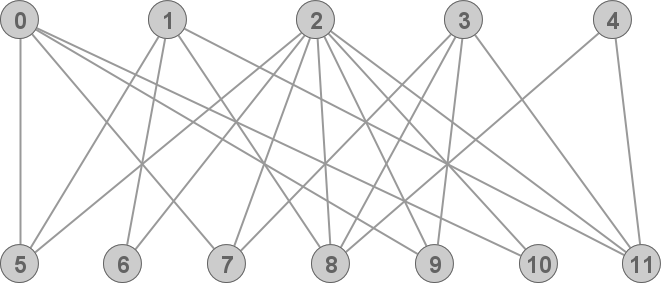
\includegraphics[scale = 0.2]{img/ej3/constructiva_golosa/bipartito1_st0.png} &
			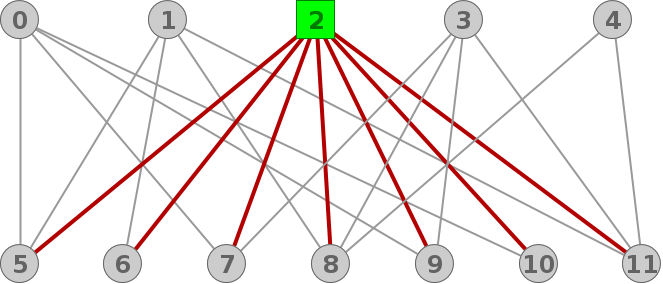
\includegraphics[scale = 0.2]{img/ej3/constructiva_golosa/bipartito1_st01.png} &
			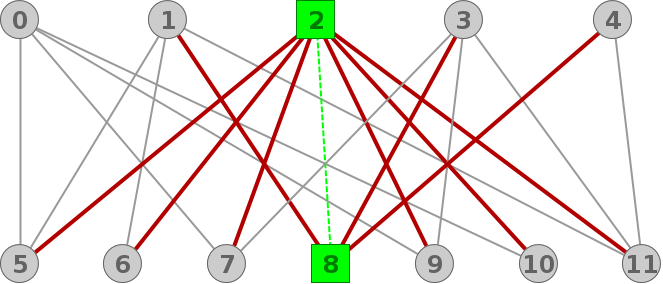
\includegraphics[scale = 0.2]{img/ej3/constructiva_golosa/bipartito1_st02.png} \\
			\hline
		\end{tabular}
	\end{center}

\subsection{Grafos circulares}
	\begin{center}
		\begin{tabular}{ |c||c| }
			\hline
			Grafo de entrada & Paso 1 \\
			\hline\hline
			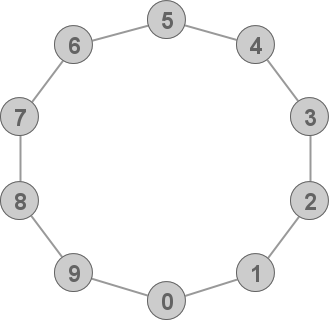
\includegraphics[scale = 0.4]{img/ej3/constructiva_golosa/Circle_st0.png} &
			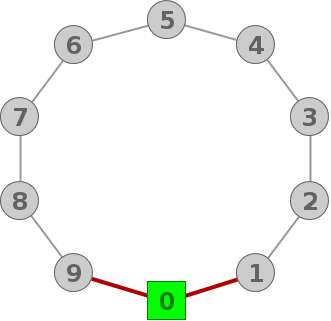
\includegraphics[scale = 0.4]{img/ej3/constructiva_golosa/Circle_st1.png} \\
			\hline
		\end{tabular}
	\end{center}

\subsection{Estrellas}
	\begin{center}
		\begin{tabular}{ |c||c| }
			\hline
			Grafo de entrada & Paso 1 \\
			\hline\hline
			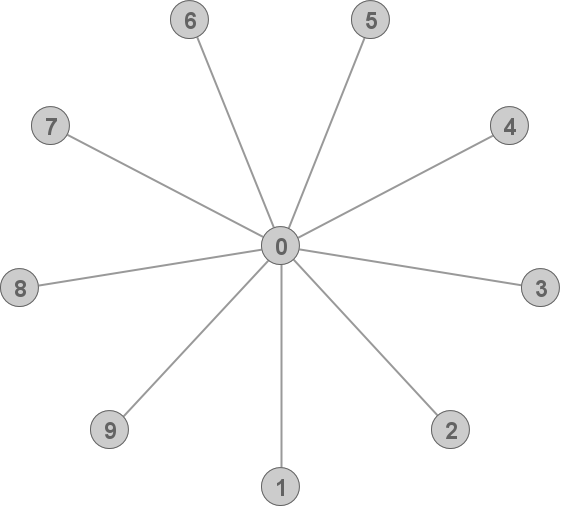
\includegraphics[scale = 0.25]{img/ej3/constructiva_golosa/Star_st0.png} &
			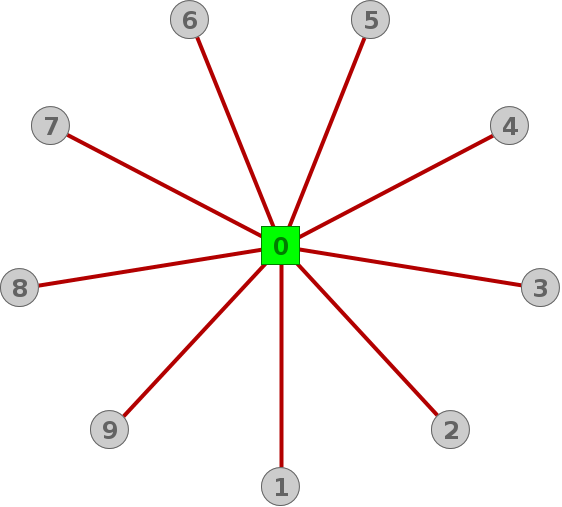
\includegraphics[scale = 0.25]{img/ej3/constructiva_golosa/Star_st1.png} \\
			\hline
		 \end{tabular}
		 \begin{tabular}{ |c||c||c| }
			\hline
			Grafo de entrada & Paso 1 & Paso 2 \\
			\hline\hline
			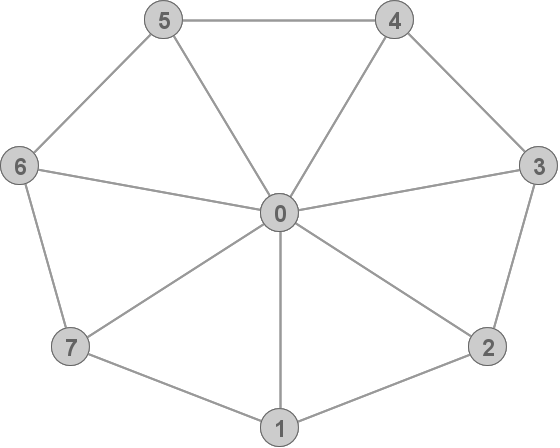
\includegraphics[scale = 0.25]{img/ej3/constructiva_golosa/Wheel_st0.png} &
			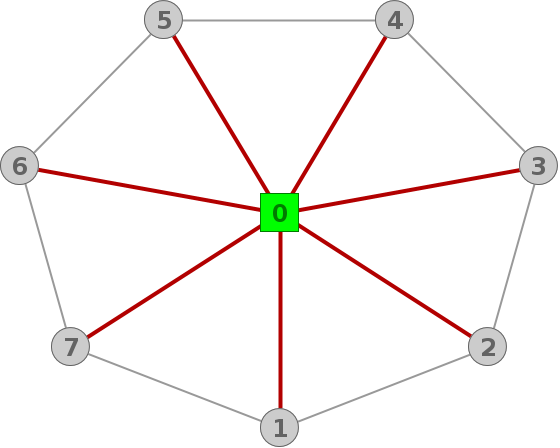
\includegraphics[scale = 0.25]{img/ej3/constructiva_golosa/Wheel_st1.png} &
			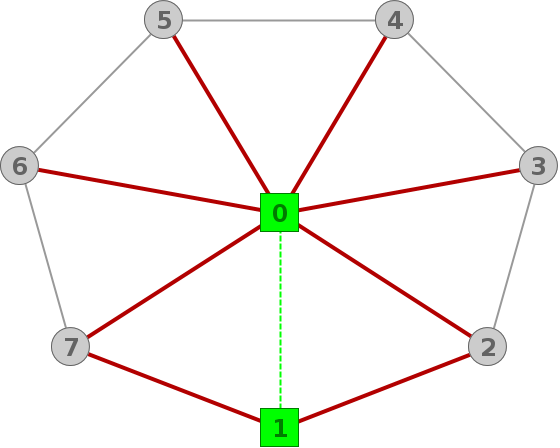
\includegraphics[scale = 0.25]{img/ej3/constructiva_golosa/Wheel_st2.png} \\
			\hline
		\end{tabular}
	\end{center}

\subsection{Grafo de secuencias}

\subsection{Banana tree}
	\begin{center}
		\begin{tabular}{ |c||c|c| }
			\hline
			Grafo de entrada & Paso 1 & Paso 2 \\
			\hline\hline
			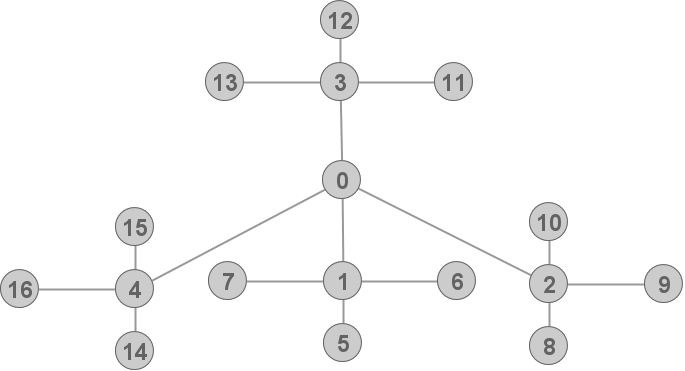
\includegraphics[scale = 0.2]{img/ej3/constructiva_golosa/banana4,4_st0.png} &
			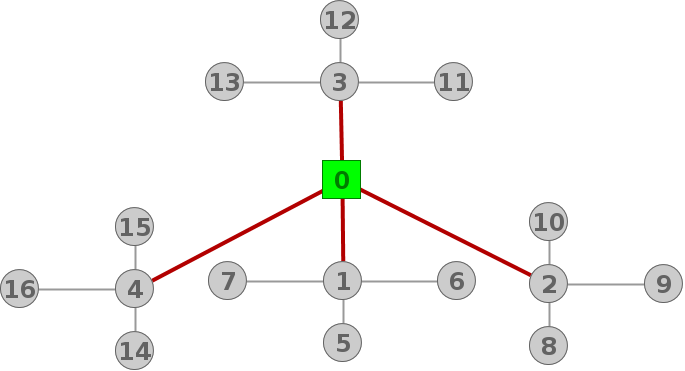
\includegraphics[scale = 0.2]{img/ej3/constructiva_golosa/banana4,4_st1.png} & 
			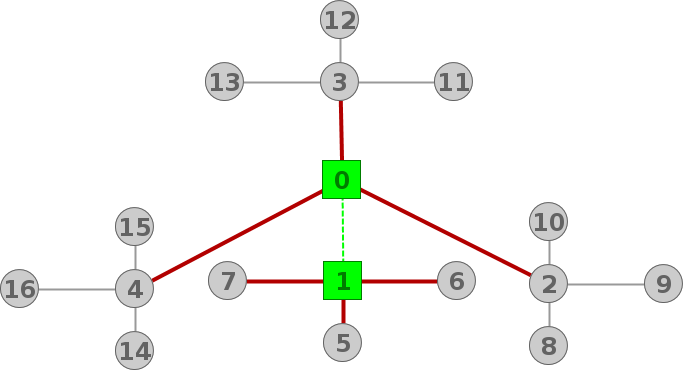
\includegraphics[scale = 0.2]{img/ej3/constructiva_golosa/banana4,4_st2.png} \\
			\hline
			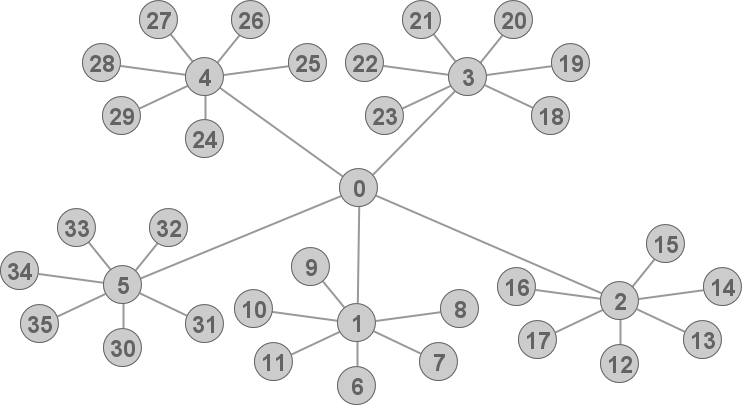
\includegraphics[scale = 0.2]{img/ej3/constructiva_golosa/banana5,7_st0.png} &
			\includegraphics[scale = 0.2]{img/ej3/constructiva_golosa/banana5,7_st1.png} &
			\includegraphics[scale = 0.2]{img/ej3/constructiva_golosa/banana5,7_st2.png} \\
			\hline
		\end{tabular}
	\end{center}




La familia de gr\'afos que asegura un resultado incorrecto de nuestra 
heur\'istica golosa puede ser caracterizada como aquella en la que el
nodo de mayor grado no forma parte de la clique de m\'axima frontera.
Esto sucede ya que la heur\'istica construye una clique a partir del 
nodo de grado m\'aximo y en cada paso se mantiene el invariante de 
de clique, agregando solamente nodos cuyo grado sea mayor al tama\~no
de la clique en ese paso, por lo tanto si alguno de los nodos de la 
clique de m\'axima frontera no forma clique con el nodo 
inicial (el de mayor grado) entonces la heuristica constructiva no 
puede llegar a incluir a ese nodo.

Ejemplos:

%\begin{tikzpicture}
%	\SetGraphUnit{1.5cm}
%	\GraphInit[vstyle=Normal]
%
%	\Vertices{circle}{2,5,6,7,8}
%	\WE(2){1}
%	\Vertices{circle}{3,10,9,11}
%	\WE(3){2}
%
%	\foreach \v in {2,5,6,7,8}{\Edge(1)(\v)};
%
%\end{tikzpicture}
	
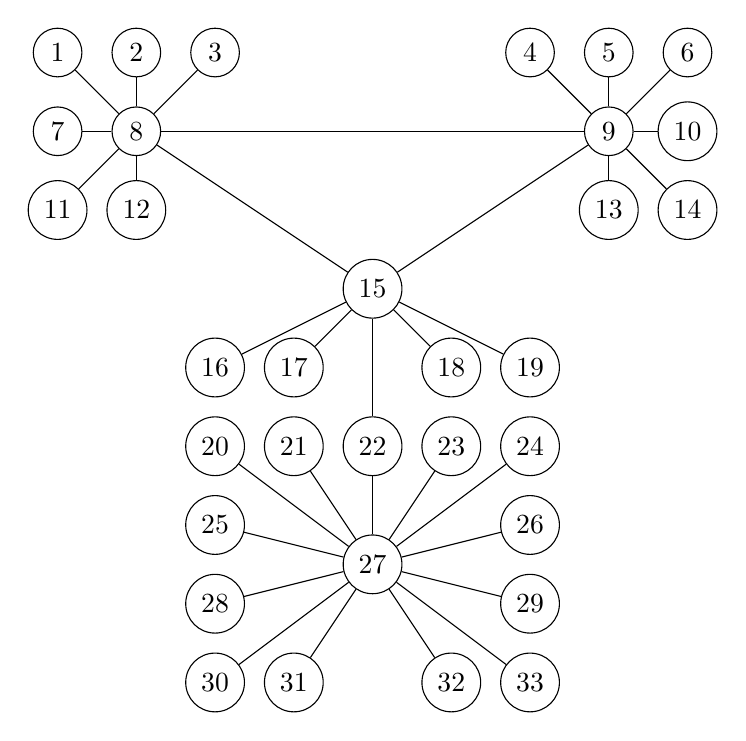
\begin{tikzpicture}
	\path 	
			% Nodos
			(0,8) node [shape=circle, draw] (1) {1}
			(1,8) node [shape=circle, draw] (2) {2}
			(2,8) node [shape=circle, draw] (3) {3}
			(6,8) node [shape=circle, draw] (4) {4}
			(7,8) node [shape=circle, draw] (5) {5}
			(8,8) node [shape=circle, draw] (6) {6}
			(0,7) node [shape=circle, draw] (7) {7}
			(1,7) node [shape=circle, draw] (8) {8}
			(7,7) node [shape=circle, draw] (9) {9}
			(8,7) node [shape=circle, draw] (10) {10}
			(0,6) node [shape=circle, draw] (11) {11}
			(1,6) node [shape=circle, draw] (12) {12}
			(7,6) node [shape=circle, draw] (13) {13}
			(8,6) node [shape=circle, draw] (14) {14}
			(4,5) node [shape=circle, draw] (15) {15}
			(2,4) node [shape=circle, draw] (16) {16}
			(3,4) node [shape=circle, draw] (17) {17}
			(5,4) node [shape=circle, draw] (18) {18}
			(6,4) node [shape=circle, draw] (19) {19}
			(2,3) node [shape=circle, draw] (20) {20}
			(3,3) node [shape=circle, draw] (21) {21}
			(4,3) node [shape=circle, draw] (22) {22}
			(5,3) node [shape=circle, draw] (23) {23}
			(6,3) node [shape=circle, draw] (24) {24}
			(2,2) node [shape=circle, draw] (25) {25}
			(6,2) node [shape=circle, draw] (26) {26}
			(4, 1.5) node [shape=circle, draw] (27) {27}
			(2,1) node [shape=circle, draw] (28) {28}
			(6,1) node [shape=circle, draw] (29) {29}
			(2,0) node [shape=circle, draw] (30) {30}
			(3,0) node [shape=circle, draw] (31) {31}
			(5,0) node [shape=circle, draw] (32) {32}
			(6,0) node [shape=circle, draw] (33) {33};
			% Aristas de la semiestrella superior izq
			\draw[-] (1) -- (8);
			\draw[-] (2) -- (8);
			\draw[-] (3) -- (8);
			\draw[-] (7) -- (8);
			\draw[-] (11) -- (8);
			\draw[-] (12) -- (8);

			% Aristas de la semiestrella superior izq
			\draw[-] (4) -- (9);
			\draw[-] (5) -- (9);
			\draw[-] (6) -- (9);
			\draw[-] (10) -- (9);
			\draw[-] (13) -- (9);
			\draw[-] (14) -- (9);

			% Mas aristas
			
			\draw[-] (8) -- (9);
			\draw[-] (8) -- (15);
			\draw[-] (9) -- (15);
			\draw[-] (16) -- (15);
			\draw[-] (17) -- (15);
			\draw[-] (18) -- (15);
			\draw[-] (19) -- (15);
			\draw[-] (22) -- (15);

			% Aristas de la estrella inferior

			\draw[-] (20) -- (27);
			\draw[-] (21) -- (27);
			\draw[-] (22) -- (27);
			\draw[-] (23) -- (27);
			\draw[-] (24) -- (27);
			\draw[-] (25) -- (27);
			\draw[-] (26) -- (27);
			\draw[-] (28) -- (27);
			\draw[-] (29) -- (27);
			\draw[-] (30) -- (27);
			\draw[-] (31) -- (27);
			\draw[-] (32) -- (27);
			\draw[-] (33) -- (27);

			
\end{tikzpicture}

\subsection{Construcci\'on de familias que rompen siempre la heur\'istica}

Intentando construir familias que siempre van a romper la heur\'istica llegamos a las siguientes
(en lo siguiente llamaremos $v$ al \'unico nodo de grado m\'aximo en un grafo):
\begin{itemize}
	\item{$v \notin CMF$}
	\item{$v \in CMF$}
\end{itemize}

Por construcci\'on estaremos viendo familias en las que existe un \'unico nodo de grado m\'aximo en el grafo.

Construyamos la primera familia que rompe la heur\'istica

\subsubsection{$v \notin CMF$}

Estamos buscando una familia de grafos en los que el nodo de grado m\'aximo no forme parte de la 
frontera, con esto en mente, partimos de un nodo de grado m\'aximo: $v$, para lograr esto $v$ ser\'a
en un principio el nodo central de una estrella. Con este escenario si la $CMF$ contuviera a $v$, la
$CMF$ ser\'ia la clique formada \'unicamente por $v$ (m\'as adelante estudiaremos como nos afecta 
relajar esta condici\'on). Como estamos viendo el caso en el que no pertenece, necesitamos una clique 
que por comodidad en un principio generaremos desconectada de $v$ para luego conectarla por 
intermedio de un puente, esto es, un camino simple entre uno de los nodos de la estrella (cualquiera
excepto $v$) y uno de los nodos de la clique al que llamaremos $v'$. 

La idea es que la $CMF$ sea parte de esa clique que agregamos, utilizamos el puente para asegurarnos
de que debido a la naturaleza de nuestra heur\'istica, esta no pueda construir una clique que contenga
a $v$ y a $v'$.

Llamemos $\Delta$ al grado de $v$, o sea la estrella tendr\'a $\Delta$ puntas. Con nuestra construcci\'on 
$v'$ puede tener a lo sumo grado $\Delta -1$, adicionalmente $v'$ es parte de una clique que luego ser\'a 
conectada por un puente a la estrella con lo que una de las aristas de $v'$ ser\'a parte del puente. 
Con esto la clique podr\'a tener a lo sumo tama\~no $\Delta -1$, dado que el grado de cada uno de los 
nodos de la clique entonces ser\'a $\Delta -2$, asegurando entonces que el grado de $v'$ no excede
el l\'imite impuesto, siempre y cuando $v'$ no tenga aristas adicionales a las que lo hacen 
parte de la clique, excepto la que lo conecta al puente.

Gr\'aficamente:
\begin{center} 
	\includegraphics[scale = 0.6]{img/ej3/constructiva_golosa/vnotincmf_carac1.png} 
\end{center}

Ahora analicemos cual es la frontera de la $CMF$: $\delta (CMF)$

Como vimos anteriormente, sabemos que la $CMF$ dentro de una clique $K_k$ tiene tama\~no
$\left\lfloor \frac{k}{2} \right \rfloor$. Tambi\'en en este caso nuestra $CMF$ deber\'a
contener a $v'$ ya que este nodo agrega una arista extra a la frontera que se puede conseguir
de cualquier clique que no lo contenga.

La frontera de esta $CMF$ asi caracterizada se calcula como la cantidad de nodos de la $CMF$
multiplicada por la cantidad de aristas que la conectan con el resto de los nodos, en este caso
(teniendo en cuenta la arista extra que conecta $v'$ con el puente):

\[ \delta(CMF) = (\left\lfloor \frac{\Delta -1}{2} \right\rfloor) \times 
	(\left\lceil \frac{\Delta -1}{2} \right\rceil) + 1 \]

Separamos en dos casos, si $\Delta$ es impar, $\Delta -1$ es par y tenemos
\[ \boxed{\delta(CMF) = (\frac{\Delta -1}{2})^2 +1} \text{ Con $\Delta$ impar} \]

si $\Delta$ es par, $\Delta -1$ es impar, llamemos $c = \frac{\Delta -1}{2}$, luego, 
$\left\lfloor c \right\rfloor = c - 1/2$ y $\left\lceil c \right\rceil = c + 1/2$ 
ambos enteros. Con esto, tenemos:
\[ \delta(CMF) = \left\lfloor c \right\rfloor \times 
	\left\lceil c \right\rceil -1 \]
\[ \delta(CMF) = (c - 1/2) \times (c + 1/2) +1 \]
\[ \delta(CMF) = c^2 - 1/4 + 1 \]
\[ \boxed{\delta(CMF) = (\frac{\Delta -1 }{2})^2 -1/4 +1} \text{ Con $\Delta$ par}\]

Del c\'alculo gen\'erico que acabamos de efectuar para la frontera de la $CMF$
podemos obtener condiciones sobre el m\'inimo $\Delta$ que necesitamos para
generar grafos de esta familia, lo que estamos buscando son los $\Delta$ que cumplen

\[ \delta(CMF) > \Delta \]

Dado que esta es la frontera de $v$ (en la estrella con la que empezamos el grafo). Resolviendo la 
inecuaci\'on para ambos casos ($\Delta$ par y $\Delta$ impar) y recordando que buscamos
enteros que cumplan esto, tenemos $\Delta \geq 6$.


Con esto el grafo con menor cantidad de nodos que cumple nuestra caracterizaci\'on ser\'a:
\begin{center} 
	\includegraphics[scale = 0.4]{img/ej3/constructiva_golosa/vnotincmf_carac1_min_st0.png} 
\end{center}

Y aqui pueden verse los resultados provistos por la heur\'istica versus los correctos:

\phantom{x}

\begin{tabular}{|c||c|}
	\hline
	Resultado obtenido por la heur\'istica & Resultado correcto \\
	\hline
	\includegraphics[scale = 0.18]{img/ej3/constructiva_golosa/vnotincmf_carac1_min_st01.png} &
	\includegraphics[scale = 0.18]{img/ej3/constructiva_golosa/vnotincmf_carac1_min_st11.png} \\
	\hline
\end{tabular}

\phantom{x}


Habiendo visto todo este proceso, podemos pensar en relajar alguna de las condiciones que 
caracterizan la familia, como por ejemplo, permitir que la estrella centrada en $v$ pase
a ser una rueda. Con esto la clique de m\'axima frontera que contiene a $v$ gana una arista, 
con lo cual para conservar la desigualdad necesitaremos que la $CMF$ encontrada
en la clique que contiene a $v'$ tambi\'en gane una arista (siempre teniendo en cuenta la
arista extra que posee $v'$ uniendolo con el puente. Se puede demostrar que empieza a
valer para $\Delta \geq 7$, pero las cuentas no agregan demasiado ya que el razonamiento
es completamente equivalente al hecho hasta ahora.

	
M\'as interesante como revelaci\'on es notar que la restricci\'on de que $v'$ est\'e
incluido en una clique de tama\~no $K_{\Delta -1}$ es demasiado fuerte. Como puede argumentarse
anal\'iticamente, pero tambi\'en puede verse diagram\'aticamente, en ese subgrafo s\'olo importa 
la cantidad de aristas de la $CMF$ con lo cual, cualquier subgrafo que conserve las restricciones
ya especificadas para la $CMF$ sigue cumpliendo las mismas relaciones n\'umericas presentadas
hasta aqu\'i y siguen rompiendo el funcionamiento de la heur\'istica. De este modo 
cualquier grafo en el que se quiten aristas de ese subgrafo original (la clique antes mencionada)
tendr\'a el mismo resultado siempre que no se quiten aristas de la $CMF$. En el caso extremo queda
la $CMF$ conectada con todos los nodos de un conjunto independiente de tama\~no 
$\left\lceil \frac{\Delta -1}{2} \right\rceil$. Diagram\'aticamente:

\begin{center} 
	\includegraphics[scale = 0.8]{img/ej3/constructiva_golosa/vnotincmf_carac2.png} 
\end{center}
